\chapter{pico2-\/ice}
\hypertarget{index}{}\label{index}\index{pico2-\/ice@{pico2-\/ice}}
\label{index_md_index}%
\Hypertarget{index_md_index}%
 \href{http://pico2-ice.tinyvision.ai/}{\texttt{ Doc}} \texorpdfstring{$\vert$}{|} \href{https://github.com/tinyvision-ai-inc/pico2-ice}{\texttt{ Hardware}} \texorpdfstring{$\vert$}{|} \href{https://github.com/tinyvision-ai-inc/pico-ice-sdk}{\texttt{ SDK}} \texorpdfstring{$\vert$}{|} \href{https://raw.githubusercontent.com/tinyvision-ai-inc/pico2-ice/docs/Board/Rev1/pico2-ice.pdf}{\texttt{ Schematic}} \texorpdfstring{$\vert$}{|} \href{https://htmlpreview.github.io/?https://github.com/tinyvision-ai-inc/pico-ice/blob/docs/Board/Rev1/bom/pico2-ice_ibom.html}{\texttt{ Assembly}} \texorpdfstring{$\vert$}{|} \href{https://discord.gg/t2CzbAYeD2}{\texttt{ Discord}}

\href{https://www.elecrow.com/pico-ice-rp2040-plus-lattice-ice40up5k-fpga.html}{\texttt{ }} \href{https://lectronz.com/stores/tinyvision-ai-store}{\texttt{ }} \href{https://www.tindie.com/stores/tinyvision_ai/?ref=offsite_badges&utm_source=sellers_vr2045&utm_medium=badges&utm_campaign=badge_small\%22\%3E}{\texttt{ }}

The pico2-\/ice is a small, low cost board with the Raspberry Pi Pico processor (\href{https://www.raspberrypi.com/documentation/microcontrollers/silicon.html\#rp2350}{\texttt{ RP2350}}) and a Lattice Semiconductor \href{https://www.latticesemi.com/en/Products/FPGAandCPLD/iCE40UltraPlus}{\texttt{ i\+CE40\+UP5K}} FPGA. The board features independent flash for the FPGA and RP2350, low power PSRAM, a couple of pushbuttons and a two 3 color LED with {\itshape all} FPGA and RP2350 pins brought out to easy to use 0.\+1"{} header pins (arranged as Pmod\textquotesingle{}s) for fast prototyping.

 
\begin{DoxyInlineImage}
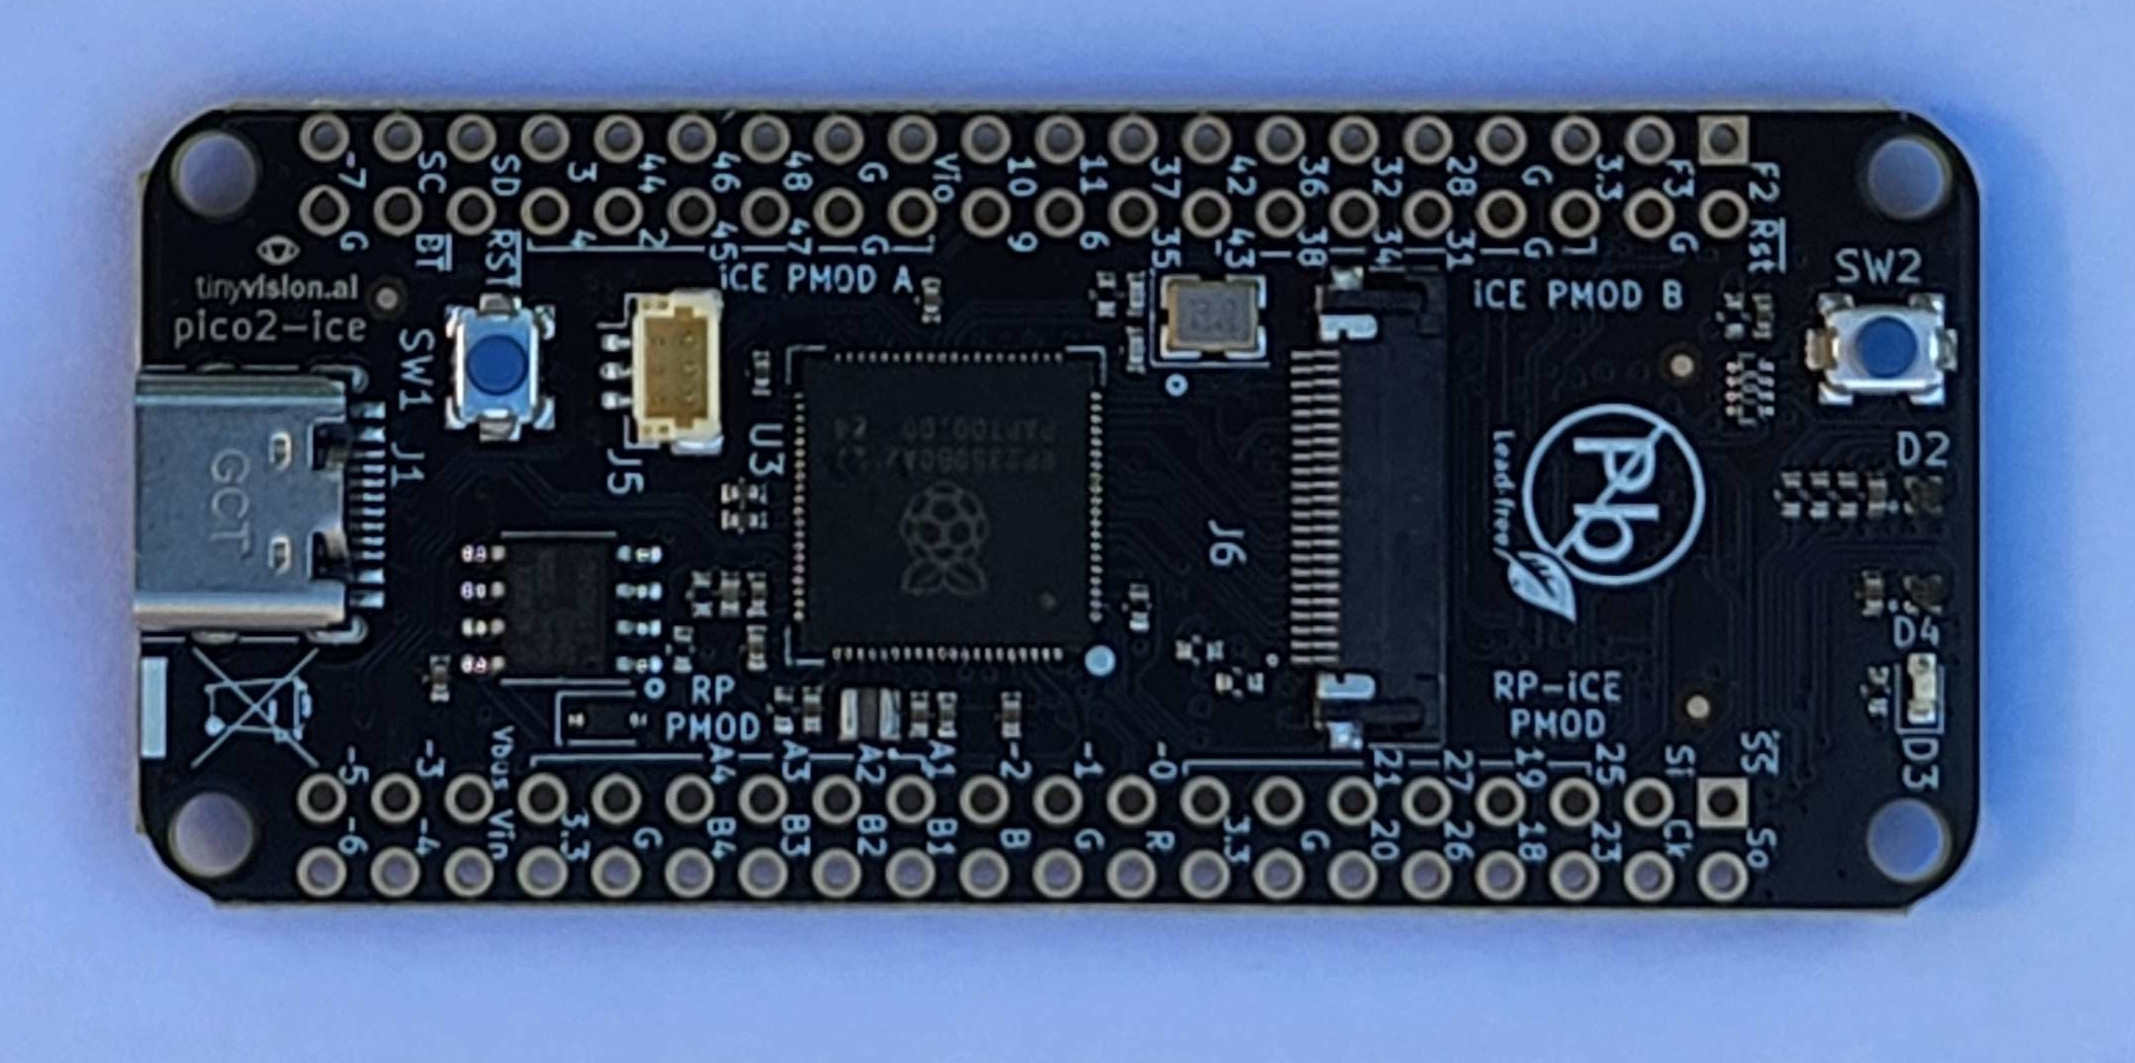
\includegraphics[height=\baselineskip,keepaspectratio=true]{pico2_ice_front.jpg}
\end{DoxyInlineImage}
   

 
\begin{DoxyInlineImage}
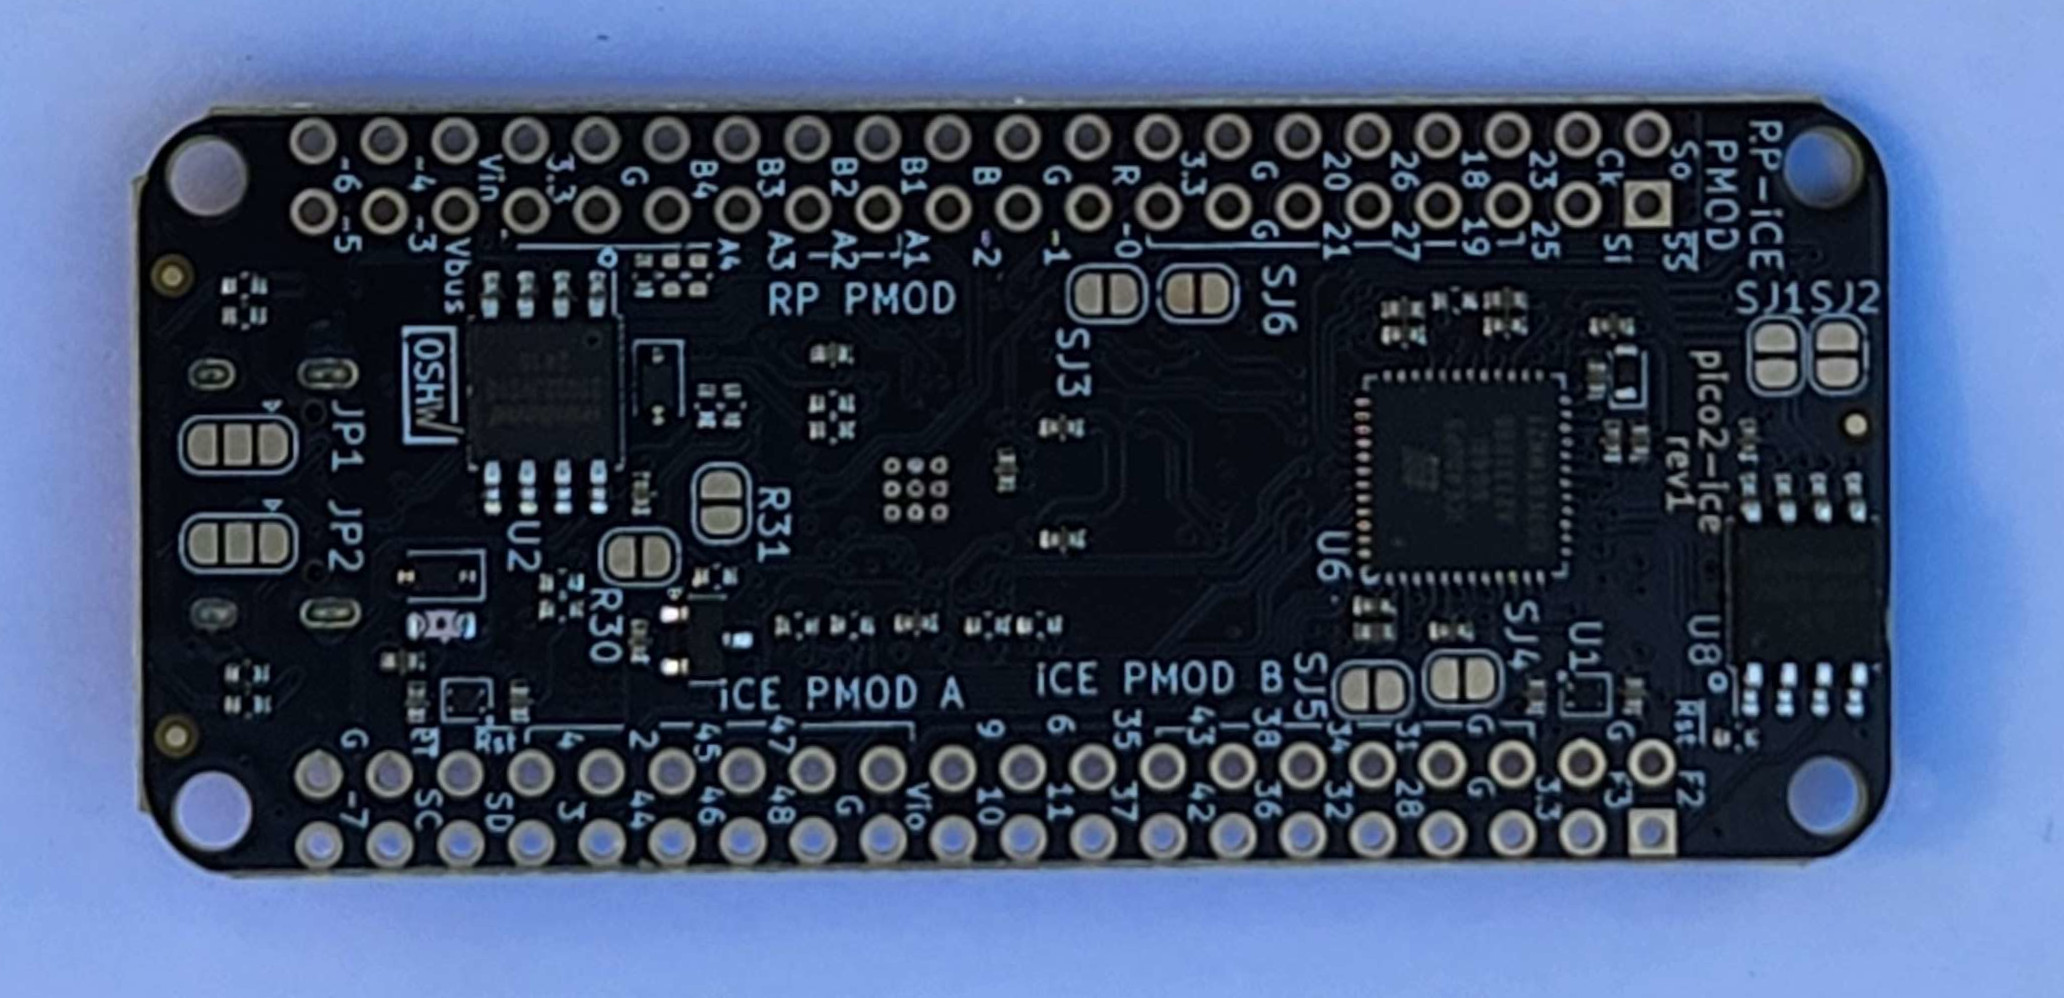
\includegraphics[height=\baselineskip,keepaspectratio=true]{pico2_ice_back.jpg}
\end{DoxyInlineImage}
   

Board Hardware Features\+:


\begin{DoxyItemize}
\item Raspberry Pi RP2350B processor
\item Lattice Ultra\+Plus ICE40\+UP5K FPGA with 5.\+3k LUTs, 1Mb SPRAM, 120Kb DPRAM, 8 Multipliers
\item {\itshape ALL} RP2350 and 32 FPGA GPIO on 0.\+1” headers
\item 4MB SPI Flash
\item 8MB low power q\+SPI SRAM
\item 2 RGB LED, one for the RP2350 and one for the FPGA
\item 2 pushbuttons, 1 for RP2350 boot mode that can also be used for other functions, and one for the FPGA
\item On board 3.\+3V and 1.\+2V Regulators, can supply 3.\+3V to your project
\item Open source schematic and layout using Ki\+CAD design tools
\item 4 layer board with a solid ground plane for good signal integrity
\end{DoxyItemize}

Board Firmware features\+:


\begin{DoxyItemize}
\item FPGA clock supplied by the RP2350, easy to program FPGA clock under SW control
\item RP2350 can program the FPGA in various ways
\end{DoxyItemize}

 
\begin{DoxyImageNoCaption}
  \mbox{\includegraphics[width=\textwidth,height=\textheight/2,keepaspectratio=true]{pico2_ice_blocks.webp}}
\end{DoxyImageNoCaption}
    